\documentclass[12pt]{article}
\usepackage{style}

\title{\textbf{The Digital Music Synthesizer}}
\author{Hanhee Lee}
\date{November 20, 2024}

\begin{document}
\maketitle
\begin{abstract}
The digital music synthesizer (DMS) is a system that makes musical sounds by using digital signal processing (DSP) techniques to (wikipedia). 
The DMS does this by modulating 
\end{abstract} 

\section{Introduction}

\section{Mathematical Background}
There are several mathematical concepts related to ECE355 that are relevant ot the DMS. These include: 


\subsection{Fourier Analysis}
From lecture
\begin{enumerate}
    \item \textbf{Synthesis Equation (Inverse Fourier Transform):}
    \begin{equation}
        x(t) = \int_{-\infty}^{\infty} X(f) e^{j 2 \pi f t} \, df
    \end{equation}

    \item \textbf{Analysis Equation (Fourier Transform):}
    \begin{equation}
        X(f) = \int_{-\infty}^{\infty} x(t) e^{-j 2 \pi f t} \, dt
    \end{equation}

\end{enumerate}

\subsection{LTI Systems}
From lecture
\begin{enumerate}
    \item \textbf{Convolution Integral in Time Domain:}
    \begin{equation}
        y(t) = (x * h)(t) = \int_{-\infty}^{\infty} x(\tau) h(t - \tau) \, d\tau 
    \end{equation}
    \item \textbf{Convolution Integral in Frequency Domain:}
    \begin{equation}
        Y(f) = X(f) \cdot H(f)
    \end{equation}
\end{enumerate}

\section{Digital Synthesis Pipeline}
\subsection{Frequency Oscillators}
The fundamental building blocks of digital music synthesis are the basic waveforms. These waveforms are used to create more complex sounds by combining them in various ways. The most common waveforms used in digital music synthesis are the sine wave, square wave, sawtooth wave, and triangle wave, 
which are created from frequency oscillators by adjusting the amplitude, frequency, and phase of the waveforms.
For $x \in \mathbb{R}^{\mathbb{R}}$ 
% MATHWORLD, PS6, https://www.antarestech.com/community/what-are-synths-in-music
\begin{enumerate}
    \item \textbf{Sine:} 
    \begin{equation}
        x(t) = A \sin(2\pi f t + \phi)
    \end{equation}
    \item \textbf{Square Wave:}
    \begin{equation}
        x(t) = \frac{1}{T} + \sum_{k \geq 1}  \frac{2}{T} \, \text{sinc} \left( \frac{k}{T} \right) \cos \left( 2 \pi \frac{k}{T} t \right)
    \end{equation}

    \begin{center}
        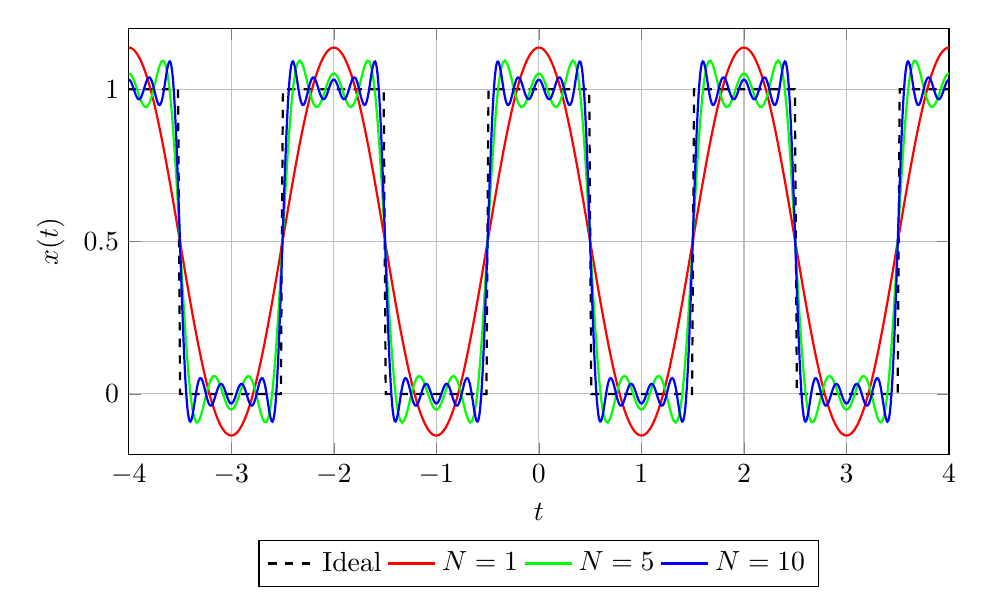
\begin{tikzpicture}
            \begin{axis}[
                width=12cm, height=7cm,
                xlabel={$t$},
                ylabel={$x(t)$},
                xmin=-4, xmax=4,
                ymin=-0.2, ymax=1.2,
                legend style={at={(0.5,-0.2)},anchor=north,legend columns=-1},
                grid=major,
                domain=-4:4,
            ]
            
            % Period T
            \def\T{2}
            
            % Ideal Square Wave
            \addplot [samples=400,black, thick, dashed, domain=-4:4] {abs(\T * round(x/\T) - x) < 0.5 ? 1 : 0};
            \addlegendentry{Ideal}
            
            % Approximation for N=1
            \addplot [samples=400,red, thick] expression {
                1/\T + (2/\T) * sin(deg(pi * 1 / \T)) / (pi * 1 / \T) * cos(deg(2 * pi * (1/\T) * x))
            };
            \addlegendentry{$N=1$}
            
            % Approximation for N=5
            \addplot [samples=400,green, thick] expression {
                1/\T 
                + (2/\T) * sin(deg(pi * 1 / \T)) / (pi * 1 / \T) * cos(deg(2 * pi * (1/\T) * x))
                + (2/\T) * sin(deg(pi * 2 / \T)) / (pi * 2 / \T) * cos(deg(2 * pi * (2/\T) * x))
                + (2/\T) * sin(deg(pi * 3 / \T)) / (pi * 3 / \T) * cos(deg(2 * pi * (3/\T) * x))
                + (2/\T) * sin(deg(pi * 4 / \T)) / (pi * 4 / \T) * cos(deg(2 * pi * (4/\T) * x))
                + (2/\T) * sin(deg(pi * 5 / \T)) / (pi * 5 / \T) * cos(deg(2 * pi * (5/\T) * x))
            };
            \addlegendentry{$N=5$}
            
            % Approximation for N=10
            \addplot [samples=1000,blue, thick] expression {
                1/\T 
                + (2/\T) * sin(deg(pi * 1 / \T)) / (pi * 1 / \T) * cos(deg(2 * pi * (1/\T) * x))
                + (2/\T) * sin(deg(pi * 2 / \T)) / (pi * 2 / \T) * cos(deg(2 * pi * (2/\T) * x))
                + (2/\T) * sin(deg(pi * 3 / \T)) / (pi * 3 / \T) * cos(deg(2 * pi * (3/\T) * x))
                + (2/\T) * sin(deg(pi * 4 / \T)) / (pi * 4 / \T) * cos(deg(2 * pi * (4/\T) * x))
                + (2/\T) * sin(deg(pi * 5 / \T)) / (pi * 5 / \T) * cos(deg(2 * pi * (5/\T) * x))
                + (2/\T) * sin(deg(pi * 6 / \T)) / (pi * 6 / \T) * cos(deg(2 * pi * (6/\T) * x))
                + (2/\T) * sin(deg(pi * 7 / \T)) / (pi * 7 / \T) * cos(deg(2 * pi * (7/\T) * x))
                + (2/\T) * sin(deg(pi * 8 / \T)) / (pi * 8 / \T) * cos(deg(2 * pi * (8/\T) * x))
                + (2/\T) * sin(deg(pi * 9 / \T)) / (pi * 9 / \T) * cos(deg(2 * pi * (9/\T) * x))
                + (2/\T) * sin(deg(pi * 10 / \T)) / (pi * 10 / \T) * cos(deg(2 * pi * (10/\T) * x))
            };
            \addlegendentry{$N=10$}
            
            \end{axis}
        \end{tikzpicture}
    \end{center}
    
    \item \textbf{Sawtooth Wave:}
    \begin{equation}
        x(t) \sum_{k \geq 1} \frac{(-1)^{k-1} T}{\pi k} \sin \left( 2 \pi \frac{k}{T} t \right)
    \end{equation}

    \begin{center}
        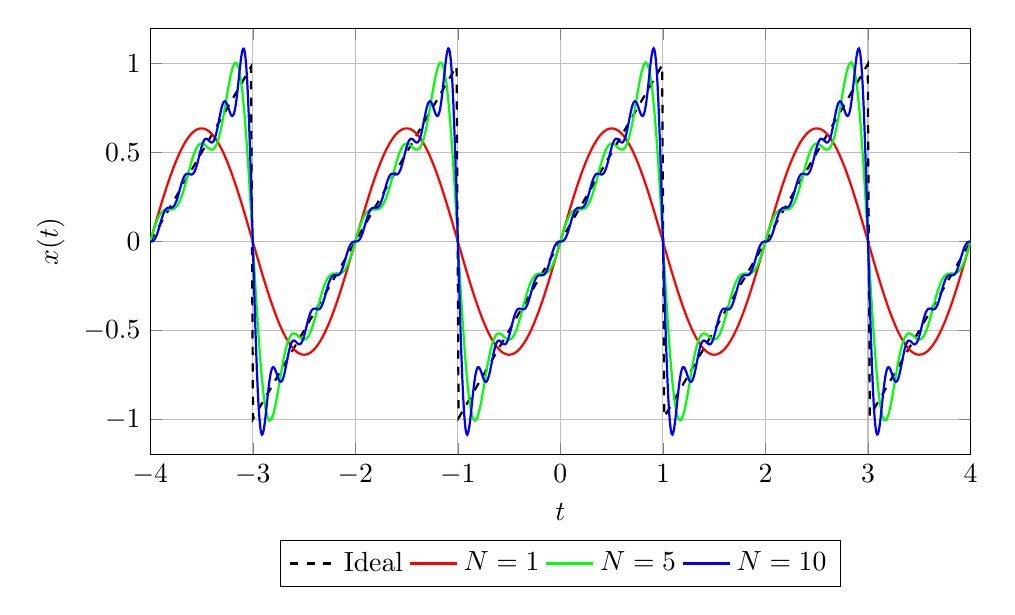
\begin{tikzpicture}
            \begin{axis}[
                width=12cm, height=7cm,
                xlabel={$t$},
                ylabel={$x(t)$},
                xmin=-4, xmax=4,
                ymin=-1.2, ymax=1.2,
                legend style={at={(0.5,-0.2)},anchor=north,legend columns=-1},
                grid=major,
                domain=-4:4,
                samples=400
            ]
            
            % Period T
            \def\T{2}
            
            % Ideal Sawtooth Wave
            \addplot [samples=400, black, thick, dashed, domain=-4:4] expression {
                2 * (x/\T - floor(0.5 + x/\T))
            };
            \addlegendentry{Ideal}
            
            % Approximation for N=1
            \addplot [samples=400, red, thick] expression {
                (-1)^0 * \T / (1 * pi) * sin(deg(2 * pi * (1/\T) * x))
            };
            \addlegendentry{$N=1$}
            
            % Approximation for N=5
            \addplot [samples=400, green, thick] expression {
                (-1)^0 * \T / (1 * pi) * sin(deg(2 * pi * (1/\T) * x))
                + (-1)^1 * \T / (2 * pi) * sin(deg(2 * pi * (2/\T) * x))
                + (-1)^2 * \T / (3 * pi) * sin(deg(2 * pi * (3/\T) * x))
                + (-1)^3 * \T / (4 * pi) * sin(deg(2 * pi * (4/\T) * x))
                + (-1)^4 * \T / (5 * pi) * sin(deg(2 * pi * (5/\T) * x))
            };
            \addlegendentry{$N=5$}
            
            % Approximation for N=10
            \addplot [samples=1000, blue, thick] expression {
                (-1)^0 * \T / (1 * pi) * sin(deg(2 * pi * (1/\T) * x))
                + (-1)^1 * \T / (2 * pi) * sin(deg(2 * pi * (2/\T) * x))
                + (-1)^2 * \T / (3 * pi) * sin(deg(2 * pi * (3/\T) * x))
                + (-1)^3 * \T / (4 * pi) * sin(deg(2 * pi * (4/\T) * x))
                + (-1)^4 * \T / (5 * pi) * sin(deg(2 * pi * (5/\T) * x))
                + (-1)^5 * \T / (6 * pi) * sin(deg(2 * pi * (6/\T) * x))
                + (-1)^6 * \T / (7 * pi) * sin(deg(2 * pi * (7/\T) * x))
                + (-1)^7 * \T / (8 * pi) * sin(deg(2 * pi * (8/\T) * x))
                + (-1)^8 * \T / (9 * pi) * sin(deg(2 * pi * (9/\T) * x))
                + (-1)^9 * \T / (10 * pi) * sin(deg(2 * pi * (10/\T) * x))
            };
            \addlegendentry{$N=10$}
            
            \end{axis}
        \end{tikzpicture}      
    \end{center}

    \item \textbf{Triangle Wave:}
    \begin{equation}
        x(t) = \sum_{k=1,3,5\ldots}^{\infty} \frac{8A}{\pi^2 k^2} (-1)^{(k-1)/2} \cos\left( 2 \pi \frac{k}{T} t \right)
    \end{equation}

    \begin{itemize}
        \item \( A \): Amplitude of the waveform.
        \item \( f [\text{Hz}]\): Frequency of the waveform.
        \item \( t \): Time.
        \item \( \phi [\text{rad}]\): Phase offset.
        \item \( n \): Harmonic number.
        \item \( T \): Period of the waveform.
    \end{itemize}
    \item \textbf{Additive Synthesis:} Synthesizing sound by adding together $N$ sinusoidal components by time-varying amplitude and frequency envelopes to get $y \in \mathbb{R}^{\mathbb{R}}$, (from Spectral audio signal processing III)
    \begin{equation}
        y(t) = \sum_{i=1}^{N} A_i(t) \sin\left(\theta_i (t)\right)
    \end{equation}
    \begin{itemize}
        \item $A_i(t) \in \mathbb{R}$: Amplitude of $i$th partial over time $t$
        \item $\theta_i (t) = \int_0^t \omega_i(t)dt + \theta_i(0) \in \mathbb{R}$
        \begin{itemize}
            \item $\omega_i(t)=\frac{d\theta_i(t)}{dt} \in \mathbb{R}$: Radian frequency of $i$th partial vs. time.
            \item $\phi_i(0) \in \mathbb{R}$: Phase offset of $i$th partial at time $0$.
        \end{itemize}
    \end{itemize}
\end{enumerate}


\subsection{Waveform Generation}
\begin{enumerate}
    \item \textbf{Subtractive Synthesis:}
    \item \textbf{Amplitude Modulation (AM) Synthesis:}
    From the theory and techniques of electronic music (Miller Puckette)
    \begin{equation}
        y(t) = A_c \left( 1 + \frac{A_m}{A_c} \cos \omega_m t \right) \cos \omega_c t
    \end{equation}

    \item \textbf{Frequency Modulation (FM) Synthesis:}
    \begin{equation}
        x(t) = A_c \sin \left[ \omega_c t + \phi_c + A_m \sin(\omega_m t + \phi_m) \right]
    \end{equation}
    
    \begin{itemize}
        \item $(A_c, \omega_c, \phi_c):$ Specify the carrier sinusoid.
        \item $(A_m, \omega_m, \phi_m):$ Specify the modulator sinusoid.
    \end{itemize}
\end{enumerate}

\subsection{Envelope Shaping}
\begin{enumerate}
    \item \textbf{Filtering:} Filtering is a method to affect only a certain range of frequencies in a signal. Some common filters are:
    \begin{itemize}
        \item \textbf{Low Pass Filter:} This filter allows low frequencies to pass through.
            $H(j2\pi f) = 
            \begin{cases} 
            1 & \text{if } |f| \leq f_c \\
            0 & \text{if } |f| > f_c 
            \end{cases}$
        \item \textbf{High Pass Filter:} This filter allows high frequencies to pass through.
            $H(j2\pi f) = 
            \begin{cases} 
            1 & \text{if } |f| \geq f_c \\
            0 & \text{if } |f| > f_c 
            \end{cases}$
        \item \textbf{Band Pass Filter:} This filter allows a certain band of frequencies to pass through.
            $H(j2\pi f) = 
            \begin{cases} 
            1 & \text{if } f_c - \frac{B}{2} \leq |f| \leq f_c + \frac{B}{2} \\
            0 & \text{otherwise} 
            \end{cases}$
    \end{itemize}


\end{enumerate}

\subsection{ADSR Envelope}


\subsection{Digital-to-Analog Conversion}
\subsubsection{Nyquist-Shannon Sampling Theorem}
% https://www.geeksforgeeks.org/nyquist-sampling-theorem/
The theorem states that a continuous signal can be reconstructed from its samples if the sampling frequency is greater than 
twice the maximum frequency of the signal:
\begin{equation}
    f_s > 2 f_{\text{max}}
\end{equation}
\begin{itemize}
    \item $f_s$: Sampling frequency.
    \item $f_{\text{max}}$: Maximum frequency of the original signal.
\end{itemize}

As a result, there are enough samples to accurately capture the details fo the signal without aliasing (i.e. distortion 
in the reconstructed signal). 
\begin{itemize}
    \item The theorem is used for Digital-to-Analog Conversion (DAC) and Analog-to-Digital Conversion (ADC). 
    \begin{itemize}
        \item Specifically, for DAC, the theorem ensures that the processed digital signal after going through the DMS pipeline can be 
        accurately converted back to an analog signal for playback through speakers or headphones. 
\end{itemize}


\subsection{Example}

\section{Conclusion}

\section*{Acknowledgement}


\begin{thebibliography}{9}  %% Organized alphabetically by author OR
                            %% in order of citation
                            %% Increase to 99 if you have more than 9 refs

\bibitem{GPSforHorseBreeding} %% a conference article
A. Akhmadiya, A. Mirmanov, N. Nabiyev, S. Bostanova, T. Serikov,
and K. Ibrayev, ``Assessing battery life and accuracy of
modern GPS trackers for herd horse breeding,'' in \emph{Proc.~2023
IEEE Int.\ Conf.\ on Smart Info.\ Sys.\ and Techn. (SIST)},
Astana, Kazakhstan, May 4--6, 2023, pp.~109--113.

\bibitem{kaplan}  %% a book
E. D. Kaplan and C. J. Hegarty, (Eds). \emph{Understanding GPS:  Principles
and Applications}, Second Edition.  Boston, MA: Artech House Publishing, 2017.

\bibitem{lewandowski} %% a journal article
W. Lewandowski, J. Azoubib, and W. J. Klepczynski, ``GPS: primary
tool for time transfer,'' \emph{Proc.\ IEEE}, vol.~87, no.~1,
pp.~163--172, Jan.~1999.

\bibitem{TamazinThesis}  %% a thesis
M. Tamazin, \emph{High Resolution Signal Processing Techniques for
Enhancing GPS Receiver Performance}, Ph.D. dissertation,
Dept.~of Electrical and Computer Engineering, Queen's University,
Kingston, Ontario, Canada, March 2015.

%% for further guidelines on reference formatting, consult the
%% IEEE Reference Guide, available online at
%% http://journals.ieeeauthorcenter.ieee.org/wp-content/uploads/sites/7/IEEE_Reference_Guide.pdf

\end{thebibliography}

\end{document}
